% !TEX TS-program = pdflatex
% !TEX encoding = UTF-8 Unicode

% This file is a template using the "beamer" package to create slides for a talk or presentation
% - Giving a talk on some subject.
% - The talk is between 15min and 45min long.
% - Style is ornate.

% MODIFIED by Jonathan Kew, 2008-07-06
% The header comments and encoding in this file were modified for inclusion with TeXworks.
% The content is otherwise unchanged from the original distributed with the beamer package.

\documentclass{beamer}


% Copyright 2004 by Till Tantau <tantau@users.sourceforge.net>.
%
% In principle, this file can be redistributed and/or modified under
% the terms of the GNU Public License, version 2.
%
% However, this file is supposed to be a template to be modified
% for your own needs. For this reason, if you use this file as a
% template and not specifically distribute it as part of a another
% package/program, I grant the extra permission to freely copy and
% modify this file as you see fit and even to delete this copyright
% notice. 


\mode<presentation>
{
  \usetheme{Warsaw}
  % or ...
  \usecolortheme{beaver}

  \setbeamercovered{transparent}
  % or whatever (possibly just delete it)
}

\usepackage[english]{babel}
% or whatever

\usepackage[utf8]{inputenc}
% or whatever

\usepackage{times}
\usepackage[T1]{fontenc}
% Or whatever. Note that the encoding and the font should match. If T1
% does not look nice, try deleting the line with the fontenc.
\usepackage{colortbl}

\title{Assignment 2}

\subtitle
{Automated Reasoning in AI 2011} % (optional)

\author{Armon Toubman, Torec Luik}

\begin{document}

\begin{frame}
  \titlepage
\end{frame}

%\begin{frame}{Outline}
%  \tableofcontents
%\end{frame}


% Since this a solution template for a generic talk, very little can
% be said about how it should be structured. However, the talk length
% of between 15min and 45min and the theme suggest that you stick to
% the following rules:  

% - Exactly two or three sections (other than the summary).
% - At *most* three subsections per section.
% - Talk about 30s to 2min per frame. So there should be between about
%   15 and 30 frames, all told.

\section{Introduction}

\subsection[General]{General Overview}

\begin{frame}{Sudoku}

\begin{table}[htbp]
        \begin{tabular}{||c|c|c||c|c|c||c|c|c||}
        \hline
        \hline
         & 9 & 4 &  &  &  & 1 & 3 & \\
        \hline
         &  &  &  &  &  &  &  & \\
        \hline
         &  &  &  & 7 & 6 &  &  & 2\\
        \hline
        \hline
         & 8 &  &  & 1 &  &  &  & \\
        \hline
         & 3 & 2 &  &  &  &  &  & \\
        \hline
         &  &  & 2 &  &  &  & 6 & \\
        \hline
        \hline
         &  &  &  & 5 &  & 4 &  & \\
        \hline
         &  &  &  &  & 8 &  &  & 7\\
        \hline
         &  & 6 & 3 &  & 4 &  &  & 8\\
        \hline
        \hline
        \end{tabular}
    \end{table}
\end{frame}

\begin{frame}{Sudoku as CSP}

  \begin{itemize}
  \item
    Variables   : Unassigned cells.
  \item
    Assignment  : Assigned cells.
  \item
    Domains     : Values 1 to 9.
  \item
    Constraints : Values 1 to 9 once in every row, column, region.
  \item
    Consistency : Constraints not violated.
  \item
    Termination : No variables left.
  \end{itemize}
\end{frame}

\begin{frame}{CSP as tree}

\begin{figure}[htbp]

\begin{center}
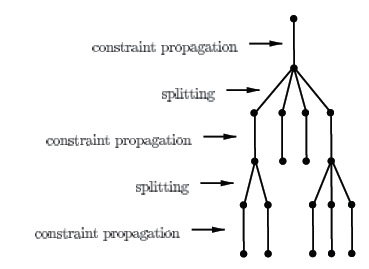
\includegraphics{tree.png}
\end{center}

\end{figure}

\end{frame}

\section{Experiment}
%%% Torec stuff
\subsection[Techniques]{Techniques}

\begin{frame}
\begin{center}
\structure{\Huge \insertsubsection}
\end{center}
\end{frame}

\begin{frame}{Tree search}

We start with the basic Depth-First Backtracking algorithm.

We add:
\begin{itemize}
\item Heuristics
\item Constraint Propagation
\end{itemize}

\end{frame}

\begin{frame}{Heuristics}

\begin{itemize}
\item From Depth-First to Best-First!
\item Heuristics
\begin{itemize}
    \item H1: Smallest domain
    \item H3: Most constrained
    \item H13: Combine H1 \& H3
\end{itemize}
\end{itemize}

\end{frame}


\begin{frame}{Constraint propagation}

\begin{itemize}
\item General
    \begin{itemize}
    \item Revise
    \end{itemize}
\item Specific
    \begin{itemize}
    \item Hidden Singles
    \item Naked Pairs
    \item Hidden Pairs
    \end{itemize}
\end{itemize}

\end{frame}

\begin{frame}{Revise}

\begin{itemize}
\item Arc consistency
\begin{itemize}
    \item Check constraints between multiple variables
\end{itemize}
\item Revise
\begin{itemize}
    \item Remove incompatible values from domains
\end{itemize}
\item AC-3
\begin{itemize}
    \item Repeat revise (intelligently) until there is no more domain reduction
\end{itemize}
\end{itemize}

\end{frame}

\begin{frame}{Revise in action}

\begin{table}[htbp]
    \begin{center}

        \begin{tabular}{|c|c|c|c|c|c|c|c|c|}
        \hline
        \cellcolor[gray]{0.7}\{1, 2, 3, 4, 5, 6, 7, 8, 9\} & 9 & 4 &  &  &  & 1 & 3 & \\
        \hline
        \end{tabular}
    \end{center}
\end{table}
\uncover<2->{
\begin{table}[htbp]
    \begin{center}

        \begin{tabular}{|c|c|c|c|c|c|c|c|c|}
        \hline
        \cellcolor[gray]{0.7}\{2, 5, 6, 7, 8\} & 9 & 4 & \{2, 5\} & \{2, 5\} & \{2, 5, 6\} & 1 & 3 & \{2, 5, 8\}\\
        \hline
        \end{tabular}
    \end{center}
\end{table}
}
\end{frame}

\begin{frame}{Hidden Singles}

\begin{table}[htbp]

    \begin{center}
        \begin{tabular}{|c|c|c|c|c|c|c|c|c|}
        \hline
        \cellcolor[gray]{0.7}\{2, 5, 6, 7, 8\} & 9 & 4 & \{2, 5\} & \{2, 5\} & \{2, 5, 6\} & 1 & 3 & \{2, 5, 8\}\\
        \hline
        \end{tabular}
    \end{center}
\end{table}
\uncover<2->{
\begin{table}
    \begin{center}

        \begin{tabular}{|c|c|c|c|c|c|c|c|c|}
        \hline
        \cellcolor[gray]{0.7}7 & 9 & 4 & \{2, 5\} & \{2, 5\} & \{2, 5, 6\} & 1 & 3 & \{2, 5, 8\}\\
        \hline
        \end{tabular}
    \end{center}
\end{table}
}

\end{frame}

\begin{frame}{Naked Pairs}

\begin{table}[htbp]

    \begin{center}

        \begin{tabular}{|c|c|c|c|c|c|c|c|c|}
        \hline
        7 & 9 & 4 & \cellcolor[gray]{0.7}\{2, 5\} & \cellcolor[gray]{0.7}\{2, 5\} & \{2, 5, 6\} & 1 & 3 & \{2, 5, 8\}\\
        \hline
        \end{tabular}
    \end{center}
\end{table}
\uncover<2->{
\begin{table}[htbp]

    \begin{center}

        \begin{tabular}{|c|c|c|c|c|c|c|c|c|}
        \hline
        7 & 9 & 4 & \{2, 5\} & \{2, 5\} & \cellcolor[gray]{0.7} 6 & 1 & 3 & \cellcolor[gray]{0.7} 8\\
        \hline
        \end{tabular}
    \end{center}
\end{table}
}
\end{frame}

\begin{frame}{Hidden Pairs}

\begin{table}[htbp]

    \begin{center}
\scalebox{0.8}{
        \begin{tabular}{|c|c|c|c|c|c|c|c|c|}
        \hline
        \cellcolor[gray]{0.7}\{2, 5, 6, 7, 8\} & 9 & 4 & \{2, 5\} & \{2, 5\} & \{2, 5, 6\} & 1 & 3 & \cellcolor[gray]{0.7}\{2, 5, 6, 7, 8\}\\
        \hline
        \end{tabular}
}
    \end{center}
\end{table}
\uncover<2->{
\begin{table}[htbp]

    \begin{center}

        \begin{tabular}{|c|c|c|c|c|c|c|c|c|}
        \hline
        \cellcolor[gray]{0.7}\{7, 8\} & 9 & 4 & \{2, 5\} & \{2, 5\} & \{2, 5, 6\} & 1 & 3 & \cellcolor[gray]{0.7}\{7, 8\}\\
        \hline
        \end{tabular}
    \end{center}
\end{table}
}
\end{frame}

%%% Armon stuff
\subsection[Results]{Results}

\begin{frame}
\begin{center}
\structure{\Huge \insertsubsection}
\end{center}
\end{frame}

\begin{frame}{Results: Optimizations}

\begin{table}
\begin{center}
\scalebox{0.7}{
\begin{tabular}{c c c c c c}
\hline
 Revise & Hidden Singles & Hidden Pairs & Naked Pairs & sudoku\_training & top95 \\
\hline
 &  &  &  & 9m49s & $*$ \\ % training_norv=589.495531305
x &  &  &  & 8m56s & 1h55m25s \\ % training_rv=536.094290474, top95_rv=6924.5242909
x & x & x & x & 25s & \cellcolor{red!50}{10s} \\ % training_rv_hs_hp_np_h13=25.511620738333335, top95_rv_hs_hp_np=9.685215524666667
x & x &  &  & 29s & 47s \\ % training_rv_hs=29.234435128, top95_rv_hs=47.415598335
x & x &  & x & \cellcolor{red!50}{23s} & 21s \\ % training_rv_hs_np=23.296235251333332,, top95_rv_hs_np=20.824697618666665
x & x & x &  & 28s & 16s \\ % training_rv_hs_hp=27.667227801666666,  top95_rv_hs_hp=15.692717729
x &   & x &  & 8m9s & 26m37s \\ % training_rv_hp=489.462033154, top95_rv_hp=1596.8818117199999
x &   & x & x & 1m21s & 3m51s \\ % training_rv_hp_np=81.19639021366667, top95_rv_hp_np=230.84322473
x &  &  & x & 1m17s & 19m32s \\ % training_rv_np=76.90551903866667, top95_rv_np=1172.4098914453334
\hline
\end{tabular}
}
\end{center}
\end{table}

\end{frame}

\begin{frame}{Results: Heuristics}

\begin{table}
\begin{center}

\scalebox{0.9}{

\begin{tabular}{c c c c c c}
\hline
 Revise & Heuristic 1 & Heuristic 3 & sudoku\_training & top95 \\
\hline
x &  &  & 8m56s & 1h55m25s \\ % training_rv=536.094290474, top95_rv=6924.5242909
x & x &  & 1m45s & 5m37s \\ % training_rv_h1=104.71135923499999, top95_rv_h1=336.839012999
x &  & x & 2m18s & 9m11s \\ % training_rv_h3=138.14704946666666, top95_rv_h3=551.151111206
x & x & x & \cellcolor{red!50}{1m45s} & \cellcolor{red!50}{9m9s} \\ % training_rv_h13=104.98554738766667, top95_rv_h13=548.8695794
\hline
\end{tabular}
}
\end{center}
\end{table}

\end{frame}

\begin{frame}{Results: Optimization + Heuristics}

\begin{table}
\begin{center}

\scalebox{0.78}{

\begin{tabular}{c c c c c c}
\hline
 Revise & Hidden Singles & Heuristic 1 & Heuristic 3 & sudoku\_training & top95 \\
\hline
x & x &  &  & 29s & 47s \\ % training_rv_hs=29.234435128, top95_rv_hs=47.415598335
x & x & x &  & \cellcolor{red!50}{25s} & 30s \\ % training_rv_hs_h1=24.783181131333333, top95_rv_hs_h1=29.532021471666667
x & x &  & x & 27s & 37s \\ % training_rv_hs_h3=26.526312118000003, top95_rv_hs_h3=37.05672543666666
x & x & x & x & \cellcolor{red!50}{26s} & \cellcolor{red!50}{26s} \\ % training_rv_hs_h13=25.561958684999997, top95_rv_hs_h13=25.992425686666667
\hline
\end{tabular}
}
\end{center}
\end{table}

\end{frame}

\begin{frame}{Best results}

\begin{table}
\begin{center}

\scalebox{1}{

\begin{tabular}{c c c c c c c c}
\hline
 Everything & sudoku\_training & top95 \\
\hline
 x & 20s & 7s \\ 
 x & 8s $*$ & 3s $*$ \\
\hline
\end{tabular}
}
\end{center}
\end{table}

\end{frame}

\section{Conclusions}

\begin{frame}{Conclusions}
\begin{itemize}
\item We created a CSP solver for the Sudoku game in Java
\item We optimized it using well-known Sudoku specific techniques
\begin{itemize}
    \item Hidden Singles
    \item Naked Pairs
    \item Hidden Pairs
\end{itemize}
\item \& general heuristics
\begin{itemize}
    \item H1 : Smallest domain
    \item H3 : Most constrained
    \item H13 : H1 \& H3 combined
\end{itemize}
\item And we got great results with all of these!
\end{itemize}
 
\end{frame}

\end{document}


